% Op icon: countersink hole — narrow channel with a conical mouth.
\documentclass[tikz,border=2mm]{standalone}
\usetikzlibrary{arrows.meta,calc,shapes.geometric}
\begin{document}
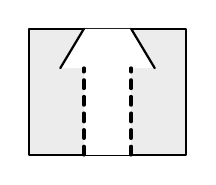
\begin{tikzpicture}[line width=1.3pt, line cap=round, line join=round, >=Stealth, x=1mm,y=1mm]
  \draw[thick, fill=gray!15] (-10,-8) rectangle (10,8);
  \fill[white] (-3,-8) rectangle (3,3);
  \fill[white] (-6,3) -- (6,3) -- (3,8) -- (-3,8) -- cycle;
  \draw[dashed] (-3,-8) -- (-3,3);
  \draw[dashed] (3,-8) -- (3,3);
  \draw[thick] (-6,3) -- (-3,8);
  \draw[thick] (6,3) -- (3,8);
\end{tikzpicture}
\end{document}
